\documentclass{article}
\usepackage[margin=1in]{geometry}
\pagenumbering{gobble}
\usepackage[utf8]{inputenc}
\usepackage{setspace}
\usepackage{multirow}
\usepackage{rotating} 
\title{Do Private Regulations `Ratchet Up?'\\
A comparative classification framework
}
\author{
Devin Judge-Lord\\
\texttt{JudgeLord@Wisc.edu}
\and
Constance L. McDermott\\
\texttt{Constance.McDermott@Ouce.Ox.ac}
\and
Benjamin Cashore\\
\texttt{Benjamin.Cashore@Yale.edu}
}
\begin{document}
\maketitle

\noindent
%\textbf{[Dear APW readers: This paper is aimed at an interdisciplinary literature across political science, economics, sociology, and management.
%that has focused more on explaining the emergence of private regulation and less on what these schemes actually require, even though many are highly complex sets of requirements, modeled on public law. 
%I am especially interested in feedback on how it could be made more interesting to an American Politics audience. Thank you!]}

\begin{abstract}
%Studies of private governance tend to deal with the conceptually and empirically challenging task of measuring differences in policy content by ``cherry-picking'' a few components, generalizing in "broad brush" strokes, or bypassing it all together. Despite, or perhaps because of, limited attention to the substance of private regulations, the last 20 years have witnessed ongoing public and scholarly debates about the ``stringency'' of various private regulations and how they change over time. However, without precise and systematic measures, it is difficult to assess these arguments. To remedy this, we offer a two-part framework. First, we focus attention on three features: policy scope; prescriptiveness; and specific policy settings. Second, these measures allow us to develop a framework for comparing regulatory systems over time, focusing on whether they are diverging, converging, or neither. We illustrate these two steps by turning to forest certification, one of the most advanced cases of global private governance. We focus on two competing programs in the United States: The Forest Stewardship Council, created by environmental advocates and their allies, and the Sustainable Forestry Initiative, created by the American Forest \& Paper Association. We find that between 2008 and 2016, these programs' regulatory standards changed little in scope but both increased in prescriptiveness. The observed patterns of ``ratcheting up'' and also maintaining or increasing relative differences, are inconsistent with prominent arguments that competition among private regulations will lead to a ``race to the bottom'' or ``convergence to the middle.'' To guide future research, we reflect on how leading theories might explain these patterns and suggest concrete steps for scholars from a range of disciplines.

% short
%Studies of private governance tend to deal with the conceptually and empirically challenging task of measuring differences in policy content by ``cherry-picking'' a few components, generalizing in ``broad brush'' strokes, or bypassing it all together. Despite, or perhaps because of, limited attention to policy substance, public and scholarly debates about the changing ``stringency'' of various private regulations persist. However, without precise and systematic measures, it is difficult to assess these arguments. To remedy this, we offer a two-part framework focusing on three policy features and potential patterns of change over time. We illustrate this framework with an analysis of two competing U.S. forest certification programs, finding that these programs changed little in scope but both increased prescriptiveness. This pattern of ``ratcheting up'' while also maintaining relative differences, is inconsistent with prominent arguments that competition among private regulations will lead to a ``race to the bottom'' or ``convergence to the middle.'' 

% version 3 
We argue that scholars must more systematically measure differences among the policies that private governance systems have developed to regulate firms. Studies of private regulations, such as product certification standards, tend to either focus on a few salient policy components, generalize in “broad brush” strokes, or bypass policy substance altogether. We show that debates over whether competing private regulations “ratchet up” or “race to the bottom” are, in part, symptoms of inconsistent measures of regulatory stringency. To remedy this, we offer a framework to systematically compare policies over time. We then apply this framework to competing activist-backed and industry-backed forestry certification programs. Our findings clarify key debates in previous scholarship but also present new puzzles: while neither program changed significantly in policy scope, both increased in prescriptiveness, albeit from different starting points, at different rates, and on different issues. The result is an overall ‘upwardly diverging’ pattern—one program targeting ecological problems and the other, industry collective action problems.
\end{abstract}

Keywords: private governance, forest certification, ecolabel, regulation, policy change




\newpage

% table 1
\begin{table}[h!]
\renewcommand{\arraystretch}{1.5} 
\centering
\caption{Concepts and Measurement of Variation in Private Regulation Content}
\label{lit}
\begin{tabular}{|l|c|c|c|}
\hline
\end{tabular}
\end{table}
\centering
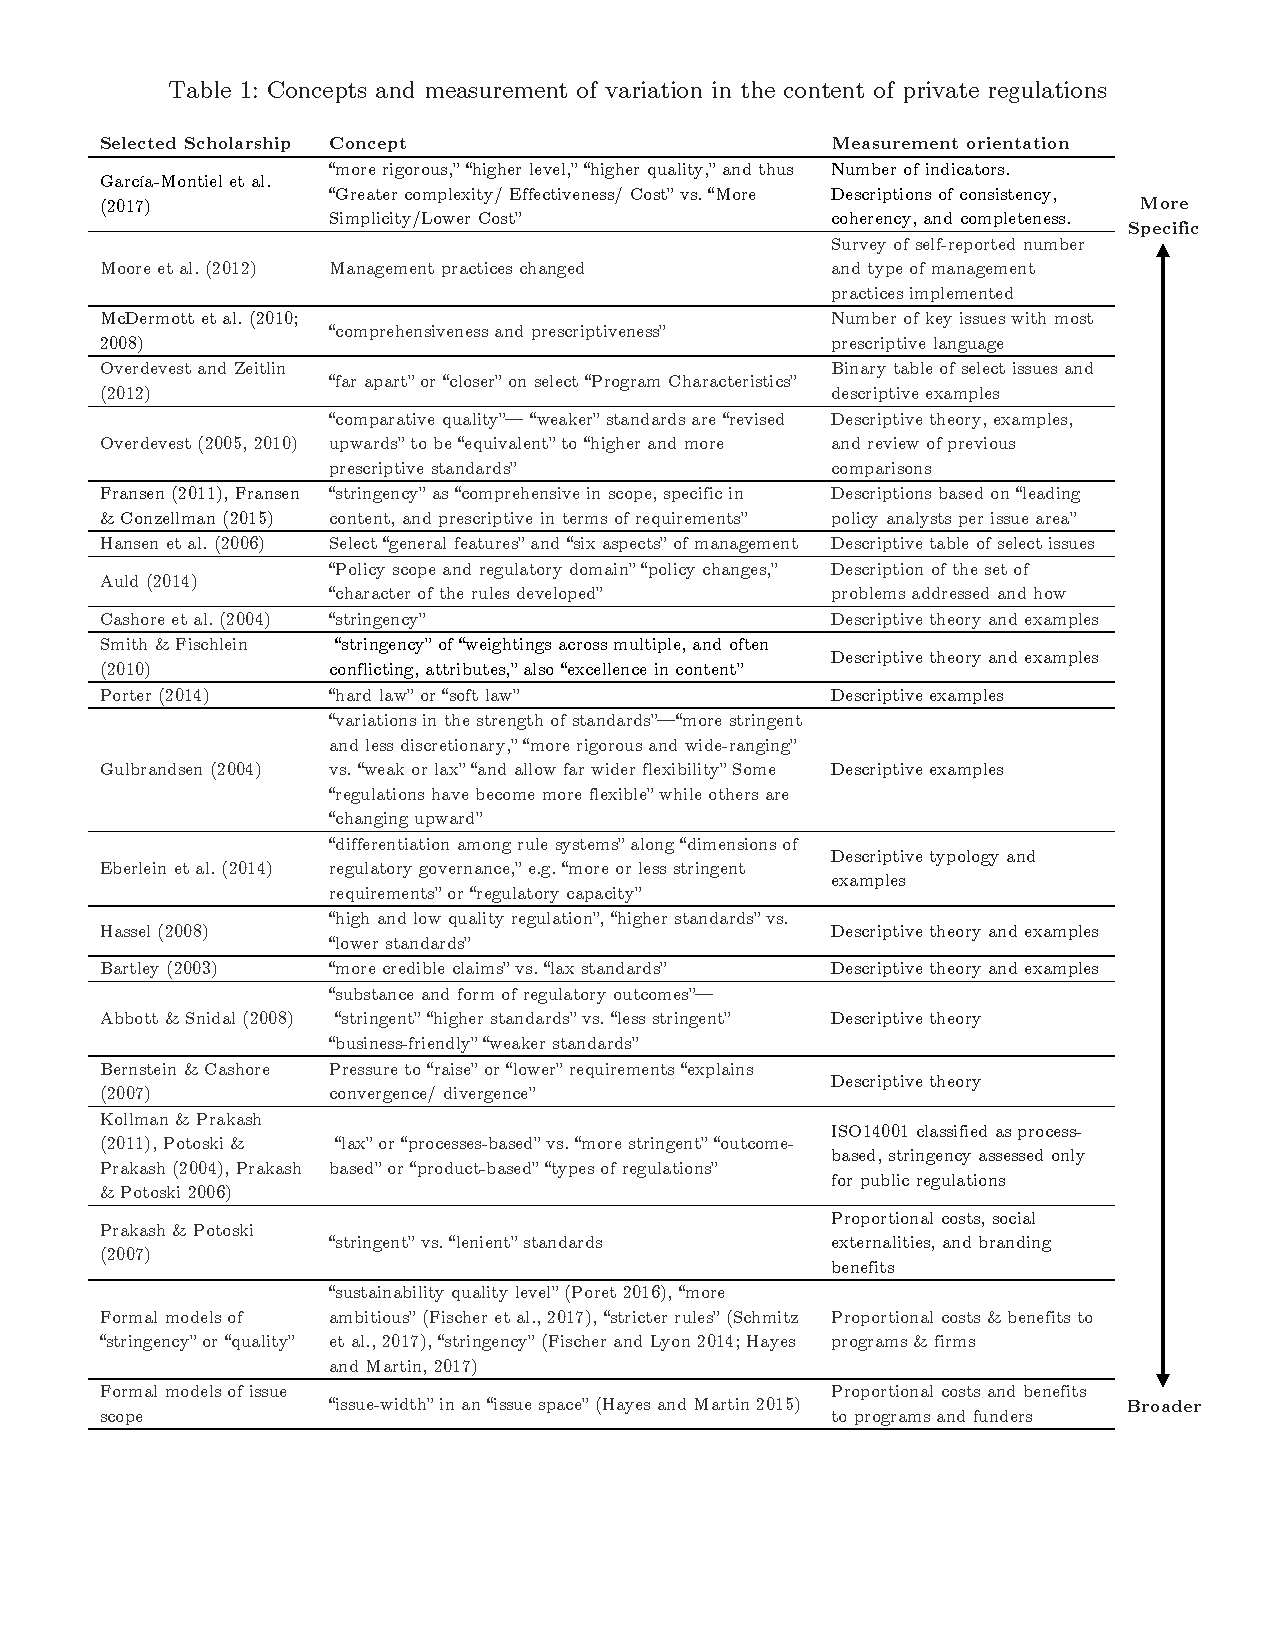
\includegraphics[trim=.5in 1in .5in .9in,clip,width = \textwidth]{table1.pdf}

\newpage

% table 2 questions
\begin{table}[h!]
\renewcommand{\arraystretch}{1.5} 
\centering
\caption{Measures of Policy Content}
\label{questions}

\end{table}
\centering
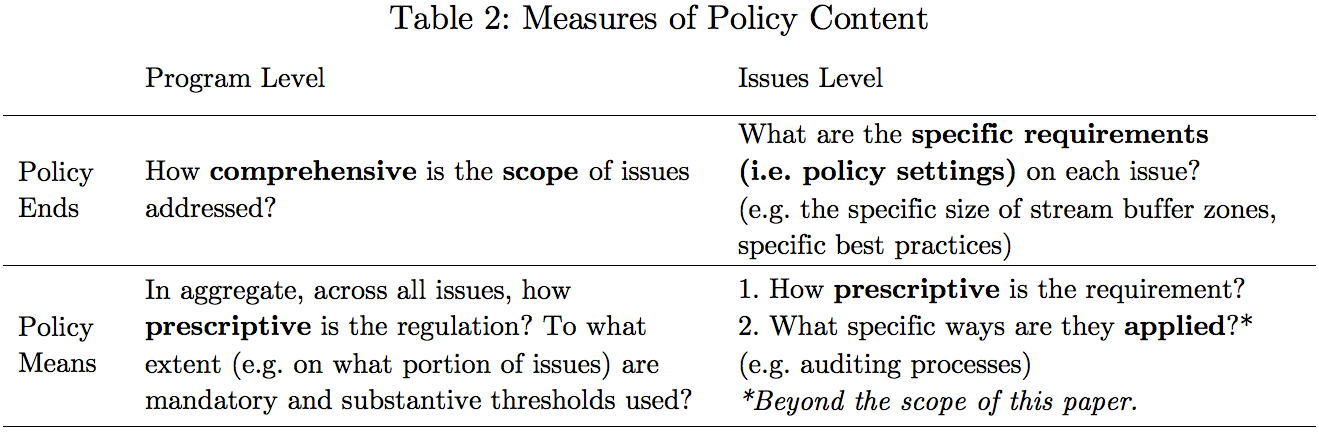
\includegraphics[trim=0 0 0 2.3cm,clip,width = \textwidth]{table2}

% table 3 prescriptiveness 
\begin{table}[h!]
\renewcommand{\arraystretch}{1.5} 
\centering
\caption{Prescriptiveness of Policy Types (adapted from Cashore (1997))}
\label{prescriptiveness}
\begin{tabular}{lccc}
 & \textbf{Discretionary} & \textbf{Non-discretionary} \\
 \cline{2-3} 
Procedural (plan- or systems-based) & Flexible & Somewhat prescriptive \\
 \cline{2-3} 
Substantive (e.g. a policy threshold) & Flexible & Most prescriptive \\
 \cline{2-3} 
\end{tabular}
\end{table}

% table 4 patterns 
\begin{figure}[h!]
\centering
\renewcommand{\arraystretch}{1.2} 
\caption{Possible Patterns of Change Among Two Private Regulations*}
\label{patterns}
\begin{tabular}{cllll}
\multicolumn{1}{c}{}                                                                                  &                               & \multicolumn{3}{c}{}                                               \\ 
\multicolumn{1}{c}{}                                                                                  &                               & \multicolumn{3}{c}{\textbf{Relationship Among Standards}}                                               \\ 
\multicolumn{1}{c}{}                                                                                  & \multicolumn{1}{c}{}         & \multicolumn{1}{c}{Converging} & \multicolumn{1}{c}{Parallel} & \multicolumn{1}{c}{Diverging} \\ \cline{3-5} 
\multicolumn{1}{c}{\multirow{6}{*}{\begin{tabular}[c]{@{}c@{}}\textbf{Directions of Change} \\ (in comprehensiveness of scope, \\prescriptiveness, \\ \textit{or} levels of requirements)\end{tabular}}} & \multicolumn{1}{c|}{Increasing}   & \multicolumn{1}{c|}{\begin{rotate}{-30}$\nearrow$\end{rotate}}           & \multicolumn{1}{c|}{$\nearrow$}       & \multicolumn{1}{c|}{$\nearrow$}          \\
\multicolumn{1}{c}{} & \multicolumn{1}{l|}{}   & \multicolumn{1}{c|}{$\nearrow$}           & \multicolumn{1}{c|}{$\nearrow$}       & \multicolumn{1}{c|}{\begin{rotate}{-30}$\nearrow$\end{rotate}}          \\
\cline{3-5} 
\multicolumn{1}{c}{} & \multicolumn{1}{c|}{Opposite or }   & \multicolumn{1}{c|}{$\searrow$}           & \multicolumn{1}{c|}{$\longrightarrow$}       & \multicolumn{1}{c|}{$\nearrow$}          \\  
\multicolumn{1}{c}{} & \multicolumn{1}{c|}{Equilibrium}   & \multicolumn{1}{c|}{$\nearrow$}           & \multicolumn{1}{c|}{$\longrightarrow$}       & \multicolumn{1}{c|}{$\searrow$}          \\ \cline{3-5} 
\multicolumn{1}{c}{} & \multicolumn{1}{c|}{} & \multicolumn{1}{c|}{$\searrow$}           & \multicolumn{1}{c|}{$\searrow$}       & \multicolumn{1}{c|}{\begin{rotate}{30}$\searrow$\end{rotate}}          \\ 
\multicolumn{1}{c}{} & \multicolumn{1}{c|}{Decreasing} & \multicolumn{1}{c|}{\begin{rotate}{30}$\searrow$\end{rotate}}           & \multicolumn{1}{c|}{$\searrow$}       & \multicolumn{1}{c|}{$\searrow$}          \\ \cline{3-5} 
\end{tabular}
\end{figure}
\footnotesize *The two arrows in each cell represent two programs. A study of three programs would have three arrows. 





\begin{figure}[h!]
\centering
\caption{Commercially-harvested Timberland in the United States}
\label{acres}
\centering
\includegraphics[width=14cm]{acres.pdf}
\centering
\footnotesize

Sources: AF\&PA, 2016; PEFC, 2017; U.S. Forest Service, 2009

%``Sustainable Forestry and Certification Programs in the United States'; US Forest Service (2009) ``Forest Resources of the United States''; PEFC (2017) ``Double certification on the rise,  joint PEFC/FSC data shows''
\end{figure}

\newpage


\begin{figure}[h!]
\centering
\label{pefc}
\caption{Comparing FSC-P\&C and PEFC on Scope and Prescriptiveness}
\includegraphics[]{fig2pefc.pdf}
\end{figure}

\newpage

\begin{figure}[h!]
\centering
\label{sfi}
\caption{Comparing FSC-US and SFI on Scope and Prescriptiveness}
\includegraphics[]{fig3sfi.pdf}
\end{figure}






\end{document}
% Please add the following required packages to your document preamble:
% \usepackage{multirow}
\begin{table}[]
\caption{Types of Policy Substance (adapted from Howlett and Cashore (2014)}
\label{my-label}
\centering

\begin{tabular}{cl|l|l|l|}
\cline{3-5}
\multicolumn{1}{c}{}                                  &                                                & \multicolumn{3}{c|}{}                                                                                                         \\ 
\multicolumn{1}{c}{}                                  &                                                & \multicolumn{3}{c|}{\textbf{Policy Content}}                                                                                                         \\ \cline{3-5} 
\multicolumn{1}{c}{}                                  &                                                & \multicolumn{1}{c|}{} & \multicolumn{1}{c|}{} & \multicolumn{1}{c|}{\textbf{}} \\ 
\multicolumn{1}{c}{}                                  &                                                & \multicolumn{1}{c|}{\textbf{High Level Abstraction}} & \multicolumn{1}{c|}{\textbf{Program Level}} & \multicolumn{1}{c|}{\textbf{Specific Measures}} \\ \hline
\multicolumn{1}{|c|}{\multirow{11}{*}{\textbf{}}} & \multirow{6}{*}{\textbf{Ends}}                 & \multicolumn{1}{c|}{\textbf{}}                  & \multicolumn{1}{c|}{\textbf{}}    & \multicolumn{1}{c|}{\textbf{}}          \\
\multicolumn{1}{|c|}{\multirow{9}{*}{\textbf{Focus}}} & \multirow{6}{*}{\textbf{}}                 & \multicolumn{1}{c|}{\textbf{GOALS}}                  & \multicolumn{1}{c|}{\textbf{OBJECTIVES}}    & \multicolumn{1}{c|}{\textbf{SETTINGS}}          \\
\multicolumn{1}{|c|}{}                                &                                                & \textbf{What general types of ideas}                 & \textbf{What does policy formally}          & \textbf{What are the specific}                  \\
\multicolumn{1}{|c|}{}                                &                                                & \textbf{govern policy development?}                  & \textbf{aim to address?}                    & \textbf{requirements?}                          \\
\multicolumn{1}{|c|}{}                                &                                                & (e.g. Conservation,                   				  & (e.g. protect ecosystems,                    & (e.g. the specific size of stream             \\
\multicolumn{1}{|c|}{}                                &                                                & Economic Development)                                & create timber processing jobs)              & buffer zones, specific best practices)                       \\ \cline{2-5} 
\multicolumn{1}{|c|}{}                                & \multirow{5}{*}{\textbf{Means}}                & \multicolumn{1}{c|}{\textbf{}}       & \multicolumn{1}{c|}{\textbf{}}    & \multicolumn{1}{c|}{\textbf{}}      \\
\multicolumn{1}{|c|}{}                                & \multirow{5}{*}{\textbf{}}                & \multicolumn{1}{c|}{\textbf{INSTRUMENT LOGIC}}       & \multicolumn{1}{c|}{\textbf{MECHANISMS}}    & \multicolumn{1}{c|}{\textbf{CALIBRATIONS}}      \\
\multicolumn{1}{|c|}{}                                &                                                & \textbf{What general norms guide policy}             & \textbf{What types of instruments}          & \textbf{What specific ways are}                 \\
\multicolumn{1}{|c|}{}                                &                                                & \textbf{implementation preferences?}                 & \textbf{are utilized?}                      & \textbf{instruments applied?}                   \\
\multicolumn{1}{|c|}{}                                &                                                & (e.g. state coercion, market demand)                 & (e.g. require processes, prescribe outcomes)& (e.g. auditing processes)                       \\ \hline
\end{tabular}
\end{table}


























\begin{table}[]
\centering
\begin{tabular}{ll|l|l|l|}
\cline{3-5}
                                             &                                                                & \multicolumn{3}{c|}{Policy Content}                                                                                                                                                                                                                                                                                                                                                                                                                                                                                                                                                                 \\ \cline{3-5} 
                                             &                                                                & High Level Abstraction                                                                                                                                                                 & Program Level Operationalization                                                                                                                                                            & Specific Measures                                                                                                                                                                                             \\ \hline
\multicolumn{1}{|c|}{\multirow{2}{*}{Focus}} & \begin{tabular}[c]{@{}l@{}}Policy Ends\\ (Aims)\end{tabular}   & \begin{tabular}[c]{@{}l@{}}GOALS\\ What general types of ideas govern policy development?\\ (e.g. Environmental Conservation, Economic Development)\end{tabular}                       & \begin{tabular}[c]{@{}l@{}}OBJECTIVES\\ What Does Policy Formally Aim to Address?\\ \\ (e.g. protect wilderness, create processing jobs)\end{tabular}                                      & \begin{tabular}[c]{@{}l@{}}SETTINGS\\ What are the specific\\ requirements?\\ (e.g. Specific size of riparian zones, harvesting levels)\end{tabular}                                                          \\ \cline{2-5} 
\multicolumn{1}{|c|}{}                       & \begin{tabular}[c]{@{}l@{}}Policy Means\\ (Tools)\end{tabular} & \begin{tabular}[c]{@{}l@{}}INSTRUMENT LOGIC\\ What general norms guide policy implementation preferences?\\ (e.g. state coersion, voluntary participation, market demand)\end{tabular} & \begin{tabular}[c]{@{}l@{}}MECHANISMS\\ What types of instruments are utilized?\\ (e.g. tax incentives, loans, public enterprise, permits, auditing and enforcement programs)\end{tabular} & \begin{tabular}[c]{@{}l@{}}CALIBRATIONS\\ What specific ways are instruments applied?\\ (e.g. who determines eligibility for incentives, rules governing trading of permits, auditing processes)\end{tabular} \\ \hline
\end{tabular}
\end{table}
